\chapter{Creación de recursos de prueba}

Con el objetivo de determinar una línea base para la creación del corpus, se inicia realizando una segmentación de recursos abiertos existentes para medir posteriormente la calidad de las segmentaciones automáticas.

Se define segmentación del audio como el proceso por medio del cual, a partir de una grabación de voz, se identifican las ocurrencias de fonemas, palabras o declaraciones. 

Se realizaron dos anotaciones para el desarrollo de la investigación: una anotación a nivel fonético y otra a nivel de declaración.

Para ambas anotaciones se utilizó el software Praat \cite{Praat} desarrollado por Paul Boersma y David Weenink de la Universidad de Ámsterdam. por medio del cual de manera visual es posible crear archivos de segmentación del audio. Estos archivos usan el formato TextGrid, especificado por la misma herramienta, donde se definen secuencias de elementos que identifican el inicio, finalización y texto encontrado en cada segmento. Estos archivos son almacenados en formato de texto para su fácil lectura \cite{TextGrids}

\section{Anotación manual a nivel fonético}

Antes de definir anotación a nivel fonético es útil definir conceptos importantes pertenecientes a la fonoaudiología para extraer información relevante para la anotación.

Se define fonema como la unidad fonológica básica, que describe una interacción específica del aparato fonador. De esta manera las posibles combinaciones finitas que puede ejecutar el ser humano para ejecutar sonidos de voz quedan acotadas por estas representaciones y a su vez son clasificadas en función de la cercanía de las interacciones.

Al ser el lenguaje hablado un subconjunto de las señales auditivas percibas por el oído como variación en la presión del aire, los primeros fonemas que destacan son aquellos que modifican directamente esta presión del aire. El aparato fonador utiliza los pulmones y el diafragma para expulsar aire, luego utiliza las cuerdas vocales, y la boca para modificar esta presión generando variaciones en los sonidos percibidos. Estos sonidos primarios son llamados vocales y se pueden caracterizar por la apertura de la boca y el lugar de resonancia de la señal.

\begin{figure}[H]
\caption{Aparato Fonador\cite{hableomsDeVoz}}
\label{img:aparato_fonador}
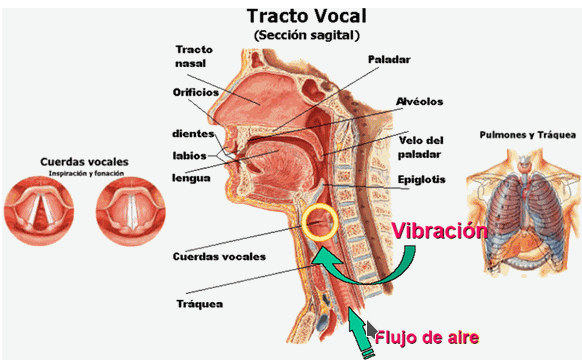
\includegraphics[width=\textwidth]{imagenes/03_02_aparato_fonador.png}
\end{figure}

El Alfabeto Fonético Internacional o IPA por sus siglas en inglés, fue estructurado desde 1888 y representa todas las posibles configuraciones para los fonemas que pueden ser ejecutados por el ser humano y la caracterización e identificación que da a las vocales es la que se puede observar en la tabla \ref{tab:ipa_table_vowels}


% \begin{landscape}
\begin{table}
\centering
\caption{Alfabeto Fonético Internacional: Vocales}
\label{tab:ipa_table_vowels}
\begin{tabular}{|l|l|l|l|l|l|l|}
\hline
{} & \multicolumn{2}{|c|}{Frontal} & \multicolumn{2}{|c|}{Central} & \multicolumn{2}{|c|}{Posterior}   \\
\hline
Cerrada & i  & y &\textbaru   & \textbari & \textturnm &  u  \\
\hline
Casi cerrada & \textsci  & \textscy &  \multicolumn{2}{|c|}{} &  & \textupsilon  \\
\hline
Semicerrada & e  & \textipa{\o} &\textreve &  \textbaro & \textramshorns & o \\
\hline
Intermedia &  \multicolumn{2}{|c|}{} & \multicolumn{2}{|c|}{\textschwa} &  \multicolumn{2}{|c|}{} \\
\hline
Semiabierta &\textepsilon  & \textipa{\oe} & \textrevepsilon & \textcloserevepsilon  & \textturnv & \textopeno \\
\hline
Casi abierta & \multicolumn{2}{|c|}{\ae} &\multicolumn{2}{|c|}{\textturna} &  \multicolumn{2}{|c|}{}  \\
\hline
Abierta & a  & \textscoelig &  \multicolumn{2}{|c|}{}  &\textscripta & \textturnscripta \\
\hline
\end{tabular}
\end{table}
% \end{landscape}

Además de estas alteraciones principales en las perturbaciones del aire, existen otros sonidos que interrumpen el flujo de aire emitido por el diafragma. Estos sonidos son denominados consonantes y son clasificados por su lugar de articulación y el tipo de articulación. El IPA también define una clasificación para las consonantes, la cual puede observarse en la tabla \ref{tab:ipa_table_pulmonic_consonants} y la tabla \ref{tab:ipa_table_non_pulmonic_consonants}

\begin{landscape}
\begin{table}
\centering
\caption{Alfabeto Fonético Internacional: Consonantes pulmónicas}
\label{tab:ipa_table_pulmonic_consonants}
\begin{tabular}{|p{25mm}|l|p{15mm}|l|l|p{15mm}|l|l|l|l|l|l|}
\hline
{} & Bilabial & Labio\newline dental & Dental & Alveolar & Post-\newline alveolar & Retrofleja & Palatal & Velar & Uvular & Faríngea & Glotal \\
\hline
Plosiva& p b  & & \multicolumn{3}{|c|}{t d} & \textipa{\:t \:d } & \textipa{c \*j} & k g &  q G & & \textipa{P} \\
\hline
Nasal& m &  \textipa{M} & \multicolumn{3}{|c|}{n} & \textipa{\:n}  &  \textipa{\*n}  & \textipa{N} & N &  & \\
\hline
Vibrante& B & & \multicolumn{3}{|c|}{r}  & & & & R &  & \\
\hline
Aproximante & & \textipa{v} & \multicolumn{3}{|c|}{\textipa{R}} & \textipa{\:r} & & & & &  \\
\hline
Fricativa  & \textipa{F B}& f v & \textipa{T D} & s z & \textipa{S z} & \textipa{\:s \:z} & \textipa{\c{c} J}& x \textipa{G} &\textipa{X  K}  &\textcrh \textipa{Q} & h\textipa{H}  \\
\hline
Lateral \newline fricative& & & \multicolumn{3}{|c|}{\textbeltl \textipa{\*z}} & & & & &  & \\
\hline
Aproximante & & \textipa{V}& \multicolumn{3}{|c|}{\textipa{\!R}} & \textipa{\:R} & j  & \textturnmrleg & & &  \\
\hline
Aproximante lateral& & \multicolumn{3}{|c|}{\textipa{l}} &  \textraisevibyi & \textturny & \textipa{\;L} & & & & \\
\hline
\end{tabular}
\end{table}
\end{landscape}

% \begin{landscape}
\begin{table}
\centering
\caption{Alfabeto Fonético Internacional: Consonantes no pulmónicas}
\label{tab:ipa_table_non_pulmonic_consonants}
\begin{tabular}{|p{20mm}|l|l|l|l|l|l|}
\hline
{} & Bilabial & Dental & Alveolar  & Palatal & Velar & Uvular   \\
\hline
Eyectiva \newline oclusiva& p\textipa{'}  & &t   & c\textipa{'} & k\textipa{'} &  q\textipa{'}  \\
\hline
Eyectiva \newline fricativa& \textipa{F'}  & \textipa{T'}&  s\textipa{'} & \textipa{\c{c}'} & x\textipa{'} & \textipa{X'}  \\
\hline
Click &\textipa{\!o}  & \textipa{|} & \textipa{!} &  & & \\
\hline
Implosiva & \textipa{\!b}  & \multicolumn{2}{|c|}{\textipa{\!d}} &  \textipa{\!j} & \textipa{\!g} & \textipa{\!G} \\
\hline
\end{tabular}
\end{table}
% \end{landscape}

El español utiliza solamente ciertos fonemas del IPA, y la representación de estos define los conocidos alfabetos fonéticos para el español. Entre los más conocidos se encuentran el SAMPA \cite{SAMPA}, y el Mexbet, el cual se representa en la tabla \ref{tab:mexbet} \cite{mexbet}.

\begin{table}[H]
\centering
\caption{Mexbet}
\label{tab:mexbet}
\begin{tabular}{|l|l|l|l|l|l|l|}
\hline
\textbf{Consonantes}         & \textbf{Labial}     & \textbf{Labio dental} & \textbf{Dental}     & \textbf{Alveolar}    & \textbf{Palatal}    & \textbf{Velar}  \\ \hline
Oclusivos Sordos             & p (p)&       & t (t)&       &       & k (k)\\ \hline
Oclusivos Sonoros            & b (b)&       & d (d)&       &       & g (g)\\ \hline
Africado Sordo               &      &       &      &       & tS (t\textipa{S}) &     \\ \hline
Fricativos Sordos            &      & f (f) &      & s (s) &       & x(x)\\ \hline
Fricativos Sonoros           &      &       &      &       & Z (\textipa{J})&     \\ \hline
Nasales                      & m (m)&       &      & n (n) & n$\sim$ (\textipa{\:n})             &     \\ \hline
Lateral                      &      &       &      & l (l) &                 & \\ \hline
Vibrante                     &      &       &      & r ({\textipa{\!R}})    &                 & \\ \hline
\end{tabular}
\end{table}

Para esto se realizó una anotación fonética manual sobre grabaciones del Open Speech Corpus \cite{Collazos2015} del subcorpus de palabras aisladas, el cual esta compuesto por 334 palabras distintas grabadas por múltiples locutores con un total de 9441 grabaciones de 39 locutores distintos, seleccionando aleatoriamente 100 palabras distintas y realizando una anotación manual por medio de PRAAT \cite{Praat}.

La anotación se realizo utilizando la convención definida en la tabla \ref{tab:anotacion_fonetica}. esta convención se uso considerando que el Open Speech corpus - words fue grabado en su totalidad por locutores latino americanos, del país Colombia y la región del Valle del Cauca. En esta representación fonética, se usa la palabra especial sil para determinar silencio; también se eliminan fonemas como la z fricativa dado que esta forma de pronunciación no es natural de la región de los hablantes.


\begin{table}[H]
\centering
\caption{Anotación Fonética}
\label{tab:anotacion_fonetica}
\begin{tabular}{|l|l|l|}
\textbf{Simbolo} & \textbf{Letra} & \textbf{Representación} \\ \hline
sil              & & Silencio                               \\ \hline
a                & a & vocal open central                   \\ \hline
b                & b &  consonante plosiva bilabial sonora   \\ \hline 
k                & c &  consonante plosiva palatal no sonora \\ \hline 
S                & ch &  consonante fricativa palatal        \\ \hline 
d                & d &  consonante plosiva dental sonora     \\ \hline 
e                & e &  vocal semi-open central              \\ \hline
f                & f &  consonante fricativa labiodental     \\ \hline 
g                & g &  consonante plosiva velar sonora      \\ \hline
i                & i &  vocal closed front                   \\ \hline
j                & j &  consonante approximant palatal       \\ \hline
l                & l &  consonante approximant alveolar      \\ \hline 
m                & m &  consonante nasal bilabial            \\ \hline 
n                & n &  consonante nasal alveolar            \\ \hline 
N                & ñ &  consonante nasal palatal             \\ \hline 
o                & o &  vocal semi-closed back               \\ \hline
p                & p &  consonante plosiva no sonora         \\ \hline 
R                & r &  consonante vibrant alveolar sonora   \\ \hline 
r                & r &  consonante vibrant alveolar no sonora \\ \hline
s                & s &  consonante fricativa alveolar         \\ \hline
t                & t &  consonante plosiva dental no sonora   \\ \hline
u                & u &  vocal closed back                    \\ \hline
y                & y &  consonante fricativa palatal         \\ \hline
\end{tabular}
\end{table}

La distribución de fonemas en la anotación manual se muestra en la tabla \ref{tab:distribucion_fonetica}

\begin{table}[H]
\centering
\caption{Distribución fonética}
\label{tab:distribucion_fonetica}
\begin{tabular}{|l|l|}
\textbf{Fonema} & \textbf{Ocurrencias} \\ \hline
sil & 173 \\ \hline
a   & 91  \\ \hline
o   & 79  \\ \hline
e   & 59  \\ \hline
n   & 45  \\ \hline
i   & 40  \\ \hline
l   & 31  \\ \hline
s   & 29  \\ \hline
t   & 27  \\ \hline
d   & 22  \\ \hline
R   & 22  \\ \hline
b   & 20  \\ \hline
r   & 19  \\ \hline
p   & 19  \\ \hline
j   & 16  \\ \hline
u   & 16  \\ \hline
m   & 15  \\ \hline
k   & 14  \\ \hline
g   & 11  \\ \hline
f   & 7   \\ \hline
c   & 5   \\ \hline
y   & 5   \\ \hline
C   & 2   \\ \hline
N   & 1   \\ \hline
S   & 1   \\ \hline
\end{tabular}
\end{table}

Las grabaciones seleccionadas se distribuyen entre 22 grabadas por locutores de género femenino, 68 masculinos y 10 no identificado.

En la imagen \ref{img:anotacion_fonetica_praat} se muestra la anotación fonética de realizada en Praat y en el archivo \ref{file:text_grid} el archivo correspondiente a la anotación fonética



\begin{figure}[H]
\caption{Anotación fonética con Praat}
\label{img:anotacion_fonetica_praat}
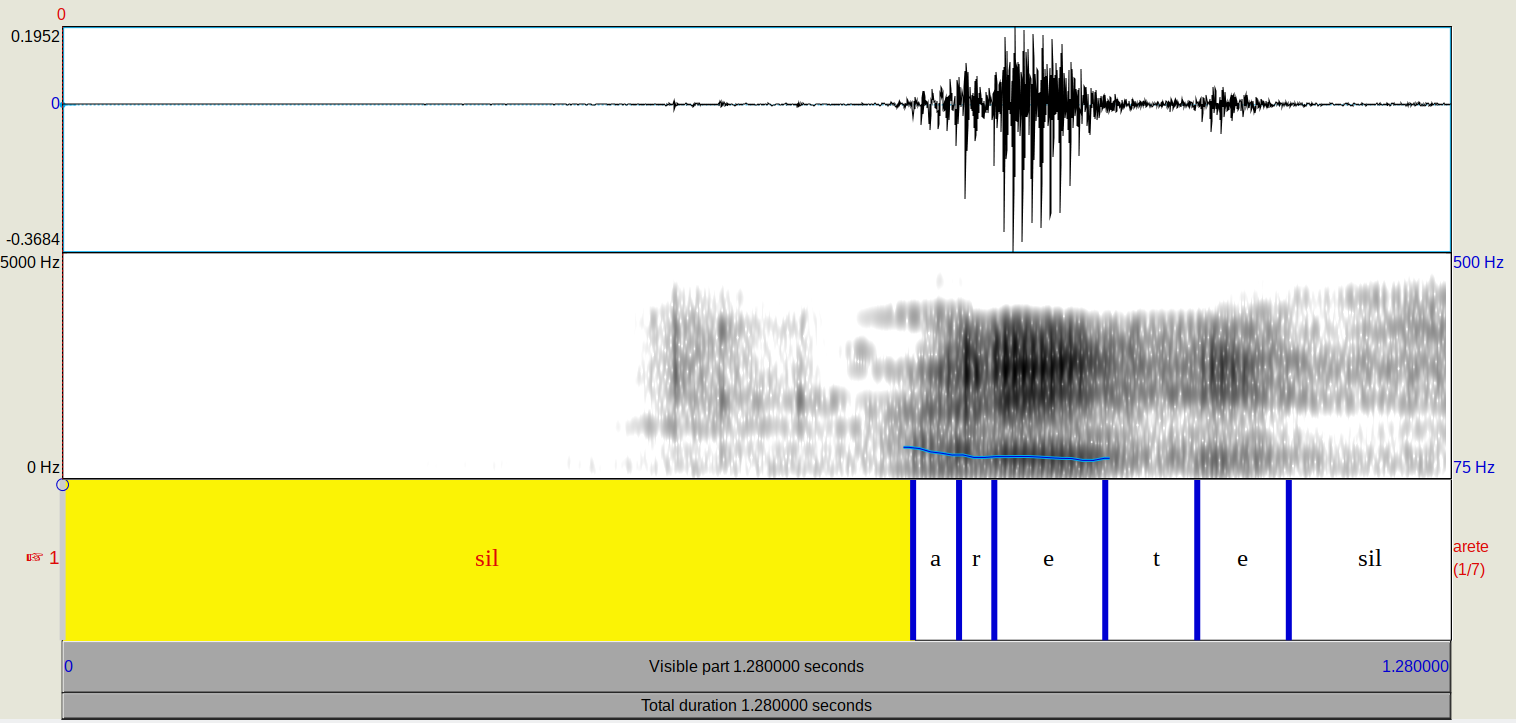
\includegraphics[width=\textwidth]{imagenes/03_01_anotacion_fonetica.png}
\end{figure}

\lstinputlisting[caption={Archivo TextGrid con anotación fonética}, label={file:text_grid}]{archivos/03_01_text_grid_ejemplo.txt}



\section{Anotación manual a nivel de sentencia}

También se realizó una anotación a nivel de declaración de los audiolibros de Librivox, seleccionando audios correspondientes a 6 horas de grabación, sobre los cuales se realizó una segmentación manual basada en símbolos de puntuación.

Para la selección de los audio libros, se ordenaron las grabaciones en orden ascendente considerando el tamaño del audio original en segundos, para posteriormente seleccionar 3 horas de locutores de género femenino y 3 horas del género masculino, garantizando de esta manera un balance de género y también la maximización de locutores diferentes. Cada archivo será identificado con un prefijo F o M que significa el género del locutor, separado por una línea baja \_ y el consecutivo asignado.

Los archivos almacenados en Librivox usan el formato de compresión con pérdida MP3, para su tratamiento son transformados a formato sin compresión WAV utilizando el programa Sox \cite{Sox}.

Se realizó de igual manera una descarga manual de los textos correspondientes a los audio libros seleccionados, generando archivos de texto plano cuya primera línea es el título del texto y el resto del archivo.

Como parte del pre-procesamiento del texto, se utilizaron expresiones regulares para segmentar los textos descargados de internet por símbolos de puntuación, y generando un nuevo archivo de texto plano donde cada línea contiene un índice, y la declaración correspondiente al segmento del texto.

Se muestra un ejemplo de texto tokenizado en el archivo \ref{file:texto_tokenizado}

\lstinputlisting[caption={Texto tokenizado}, label={file:texto_tokenizado}]{archivos/03_02_tokenizacion_texto.txt}

Los índices al comienzo de cada línea funcionan como identificadores en el proceso de anotación a nivel de declaración. Esto con el objetivo de facilitar el proceso de anotación al solo indicar en el campo de texto un índice en lugar del texto correspondiente. Posteriormente es posible reconstruir un archivo de anotación, reemplazando los índices por el texto correspondiente almacenado en el archivo de tokenización. El ejemplo de anotación de declaración del texto ejemplo se puede observar en el archivo \ref{file:text_grid_tokenizado}

\lstinputlisting[caption={Texto tokenizado}, label={file:text_grid_tokenizado}]{archivos/03_03_text_grid_tokenizado.txt}


\section{Anotación automática a nivel de sentencia usando Libri Vox Spanish}

\textcolor{red}{WIP}

Esta sección corresponde a la generación de TextGrids usando los archivos fuentes descargados directamente desde librivox y comparándolos con la segmentación manual de \cite{LibriVox-Spanish}, de momento no tengo nada acá mas que experimentos fallidos usando Onsets y de pronto luego miro si hay tiempo de dejar este capítulo si encuentro alguna luz. De pronto usando DTW pasa algo acá pero no se.

